\documentclass[hidelinks,a4paper,12pt, nofootinbib]{article}
\usepackage[width=15.5cm, left=3cm, top=2.5cm, right=2cm, left=2cm, height= 24.5cm]{geometry}
\usepackage[spanish, es-tabla]{babel} %es-tabla es para que ponga Tabla en vez de Cuadro en el caption
\usepackage[utf8]{inputenc}
\usepackage[T1]{fontenc}
\usepackage{xspace}
\usepackage{xargs}
\usepackage{fancyhdr}
\usepackage{lastpage}
\usepackage{caratula}
\usepackage[bottom]{footmisc}
\usepackage{amsmath}
\usepackage{amssymb}
\usepackage{algorithm}
\usepackage[noend]{algpseudocode}
\usepackage{array}
\usepackage{xcolor,colortbl}
\usepackage{amsthm}
\usepackage{listings}
\usepackage{soul}

\usepackage{pgf}

\usepackage{graphicx}
\usepackage{sidecap}
\usepackage{wrapfig}
\usepackage{caption}

%Grafos
\usepackage{tkz-berge} %Como Tikz pero más orientado a graph theory 
\usetikzlibrary{3d,arrows,automata,shapes,snakes}
\newcommand\pgfmathsinandcos[3]{% 
  \pgfmathsetmacro#1{sin(#3)}% 
  \pgfmathsetmacro#2{cos(#3)}% 
}


%Formato de los links
\usepackage{hyperref}
\hypersetup{
  colorlinks   = true, %Colours links instead of ugly boxes
  urlcolor     = blue, %Colour for external hyperlinks
  linkcolor    = blue, %Colour of internal links
  citecolor   = red %Colour of citations
}

\usepackage{comment}

\captionsetup[table]{labelsep=space}


\setlength{\parindent}{4em}
\setlength{\parskip}{0.5em}


%%fancyhdr
\pagestyle{fancy}
\thispagestyle{fancy}
\addtolength{\headheight}{1pt}
\lhead{Inferencia Bayesiana con Aplicaciones en Ciencias Cognitivas}
\rhead{$1º$ cuatrimestre de 2016}
\cfoot{\thepage\ / \pageref{LastPage}}
\renewcommand{\footrulewidth}{0.4pt}
\renewcommand{\labelitemi}{$\bullet$}

%%caratula
\materia{Inferencia Bayesiana}
\titulo{Trabajo Práctico}
%\subtitulo{}
%\grupo{Grupo 12}
\integrante{Costa, Manuel José Joaquín}{035/14}{manucos94@gmail.com}
\integrante{Gatti, Mathias Nicolás}{477/14}{mathigatti@gmail.com}

\fecha{26 de Mayo de 2016}

\usepackage{etoolbox}
\AtBeginEnvironment{tikzpicture}{\shorthandoff{>}\shorthandoff{<}}{}{}

\begin{document}
\maketitle

\tableofcontents
\newpage


\section{Ejercicio 1}
El modelo que escogimos se describe a continuación, en este entran en juego distintos parametros de distribuciones que modelan el problema y datos obtenidos que nos ayudaran a predecir mejor las distribuciones de los parámetros. Los cálculos de inferencia se realizaran con JAGS. Mas adelante se describe el código utilizado en el código del modelo.

\begin{figure}[H]
\begin{minipage}{0.5\textwidth}
\centering
\begin{tikzpicture}[>=stealth', shorten >=1pt,auto,node distance=1.9cm,
                    semithick]
  \tikzstyle{every state}=[fill=white,draw=black,text=black]

	\node[state, rectangle]	(0)							{$\alpha$};
	\node[state]				(1) [right of=0, below of=0]	{$\theta_3$};
	\node[state]				(3) [left of=0, below of=0]	{$\theta_1$};
	\node[state]				(2) [below of=0] 			{$\theta_2$};
	\node[state, rectangle]	(5) [below of=2, fill=gray] 	{$k_2$};
	\node[state, rectangle]	(4) [below of=1, fill=gray]	{$k_3$};
	\node[state, rectangle]	(6) [below of=3, fill=gray] 	{$k_1$};
	\node[state, rectangle]	(7) [below of=5, fill=gray] 	{$n$};

	\path[->]	
			(0) edge  []						node {} (1)
				edge  []						node {} (2)
				edge	  []						node {} (3)			
			(1) edge  []  					node {} (4)
			(2) edge  []						node {} (5)
			(3)	edge  [] 					node {} (6)
			(7) edge  []  					node {} (4)
				edge  []						node {} (5)
        			edge  [] 					node {} (6);

\end{tikzpicture}
\end{minipage}%
\begin{minipage}{0.5\textwidth}

$\beta \sim Categorical(pi)$

$
  \theta_1 \sim
\begin{cases}
  Beta(0.5,0.5)	& \text{if}\ \beta = 1 \\
  Beta(100,100)	& \text{if}\ \beta \neq 1
\end{cases}
$

$ k_1 \sim Binomial(\theta_1,n) $

$ k_2 \sim Binomial(\theta_2,n) $

$ k_3 \sim Binomial(\theta_3,n) $

$ n = 10  $

\end{minipage}
\end{figure}

\begin{lstlisting}[frame=single]
model{  
	# Observed Counts
	k1 ~ dbin(theta1,n)
	k2 ~ dbin(theta2,n)
	k3 ~ dbin(theta3,n)

	# Prior on Rates Theta
	theta1 ~ dbeta(param1, param1)
	theta2 ~ dbeta(param2, param2)
	theta3 ~ dbeta(param3, param3)

	# Auxiliary variables for Theta's distribution
	param1 <- ifelse(alpha== 1, 0.5, 100)
	param2 <- ifelse(alpha== 2, 0.5, 100)
	param3 <- ifelse(alpha== 3, 0.5, 100)

	# Prior on Rate Alpha
	for( i in 1:3){
	pi[i] <- 1/3
	}
	alpha ~ dcat(pi[])	
}
\end{lstlisting}



\newpage

\section{Ejercicio 2}
Como valores iniciales de las variables no observadas escogimos distintas opciones para asegurarnos de que no haya diferencia en los valores a los cuales convergen. Para los gráficos expuestos se utilizaron los siguientes parámetros para el algoritmo de muestreo.

\begin{lstlisting}[frame=single]
% Sampling
% MCMC Parameters
nchains = 2; % How Many Chains?
nburnin = 10e2; % How Many Burn-in Samples?
nsamples = 10e4;  %How Many Recorded Samples?
nthin = 1; % How Often is a Sample Recorded?
doparallel = 0; % Parallel Option

% Assign Matlab Variables to the Observed Nodes
datastruct = struct('k1',k1,'k2',k2,'k3',k3,'n',n);

% Initialize Unobserved Variables
for i=1:nchains
    S.theta1 = 0.5; % Intial Value
    S.theta2 = 0.8; % Intial Value
    S.theta3 = 0.5; % Intial Value
    S.alpha = randi([1 3]); % Intial Value
    init0(i) = S;
end

\end{lstlisting}

\subsection{Histogramas}

\begin{figure}[H]
\begin{minipage}{0.5\textwidth}
 \centering
	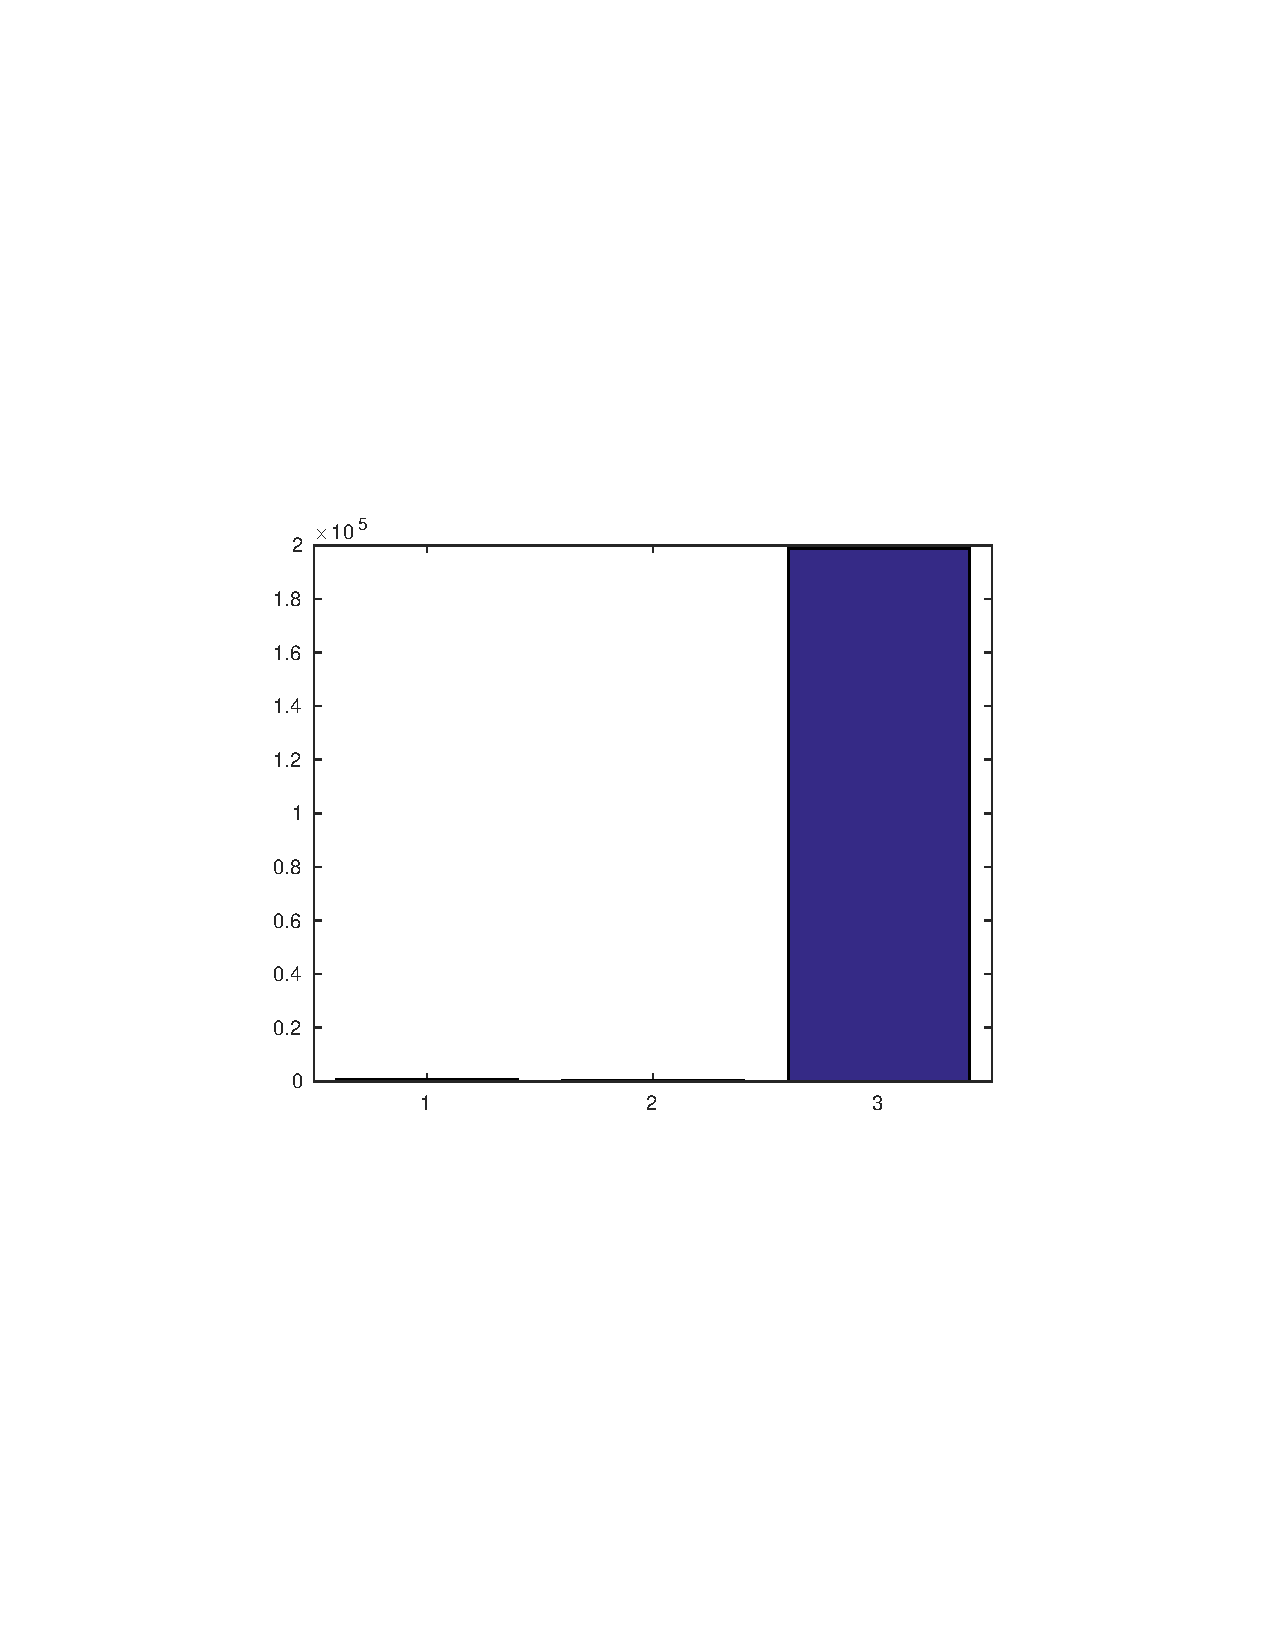
\includegraphics[width=1.2\textwidth]{imgs/alpha.pdf}
	\caption{\footnotesize Histograma de la variable $\alpha$.}
\end{minipage}
\begin{minipage}{0.5\textwidth}
 \centering
	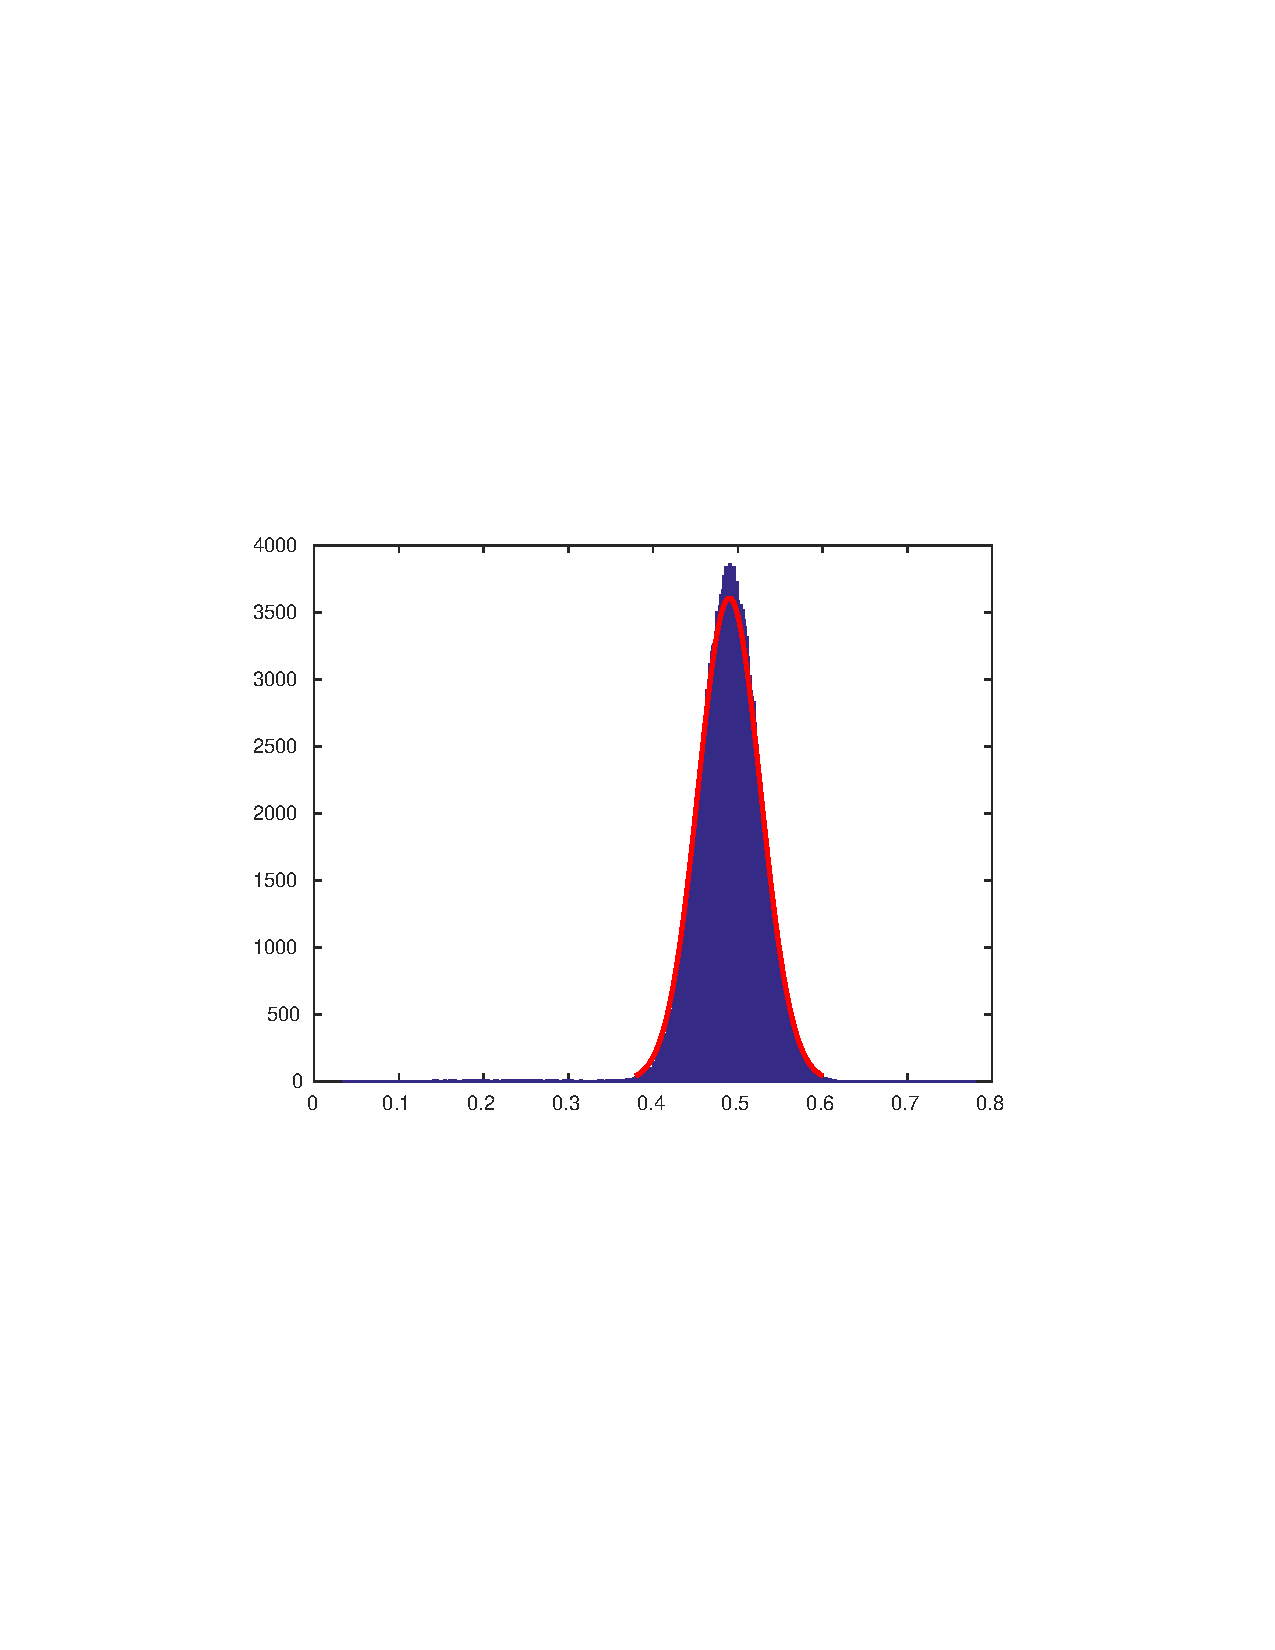
\includegraphics[width=1.2\textwidth]{imgs/theta1.pdf}
	\caption{\footnotesize Histograma de la variable $\theta_1$. La linea azul es una aproximacion con una distribución normal.}
\end{minipage}
\end{figure}


\begin{figure}[H]
\begin{minipage}{0.5\textwidth}
 \centering
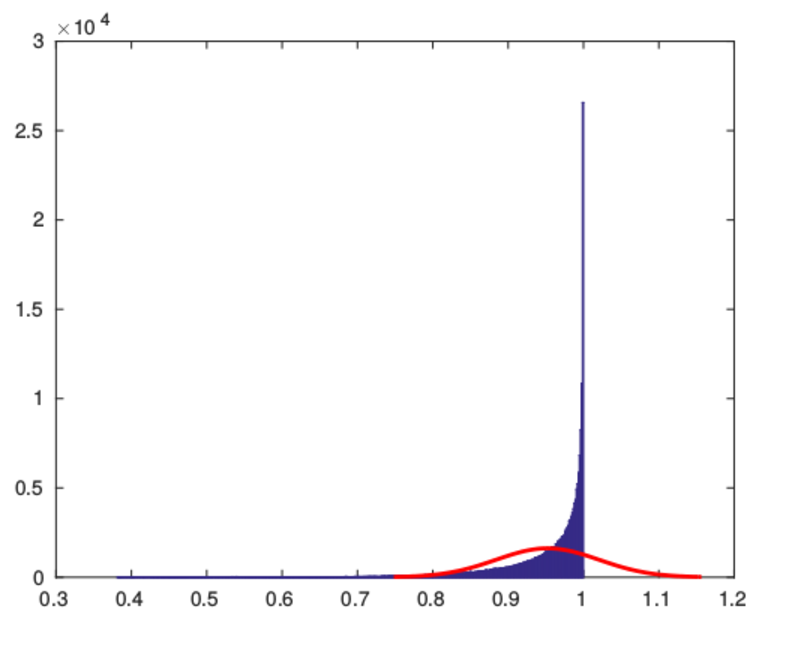
\includegraphics[width=0.9\textwidth]{imgs/theta3.pdf}
	\caption{\footnotesize Histograma de la variable $\theta_3$. La linea azul es una aproximacion (Poco precisa como se podrá observar)con una distribución normal.}
\end{minipage}
\begin{minipage}{0.5\textwidth}
 \centering
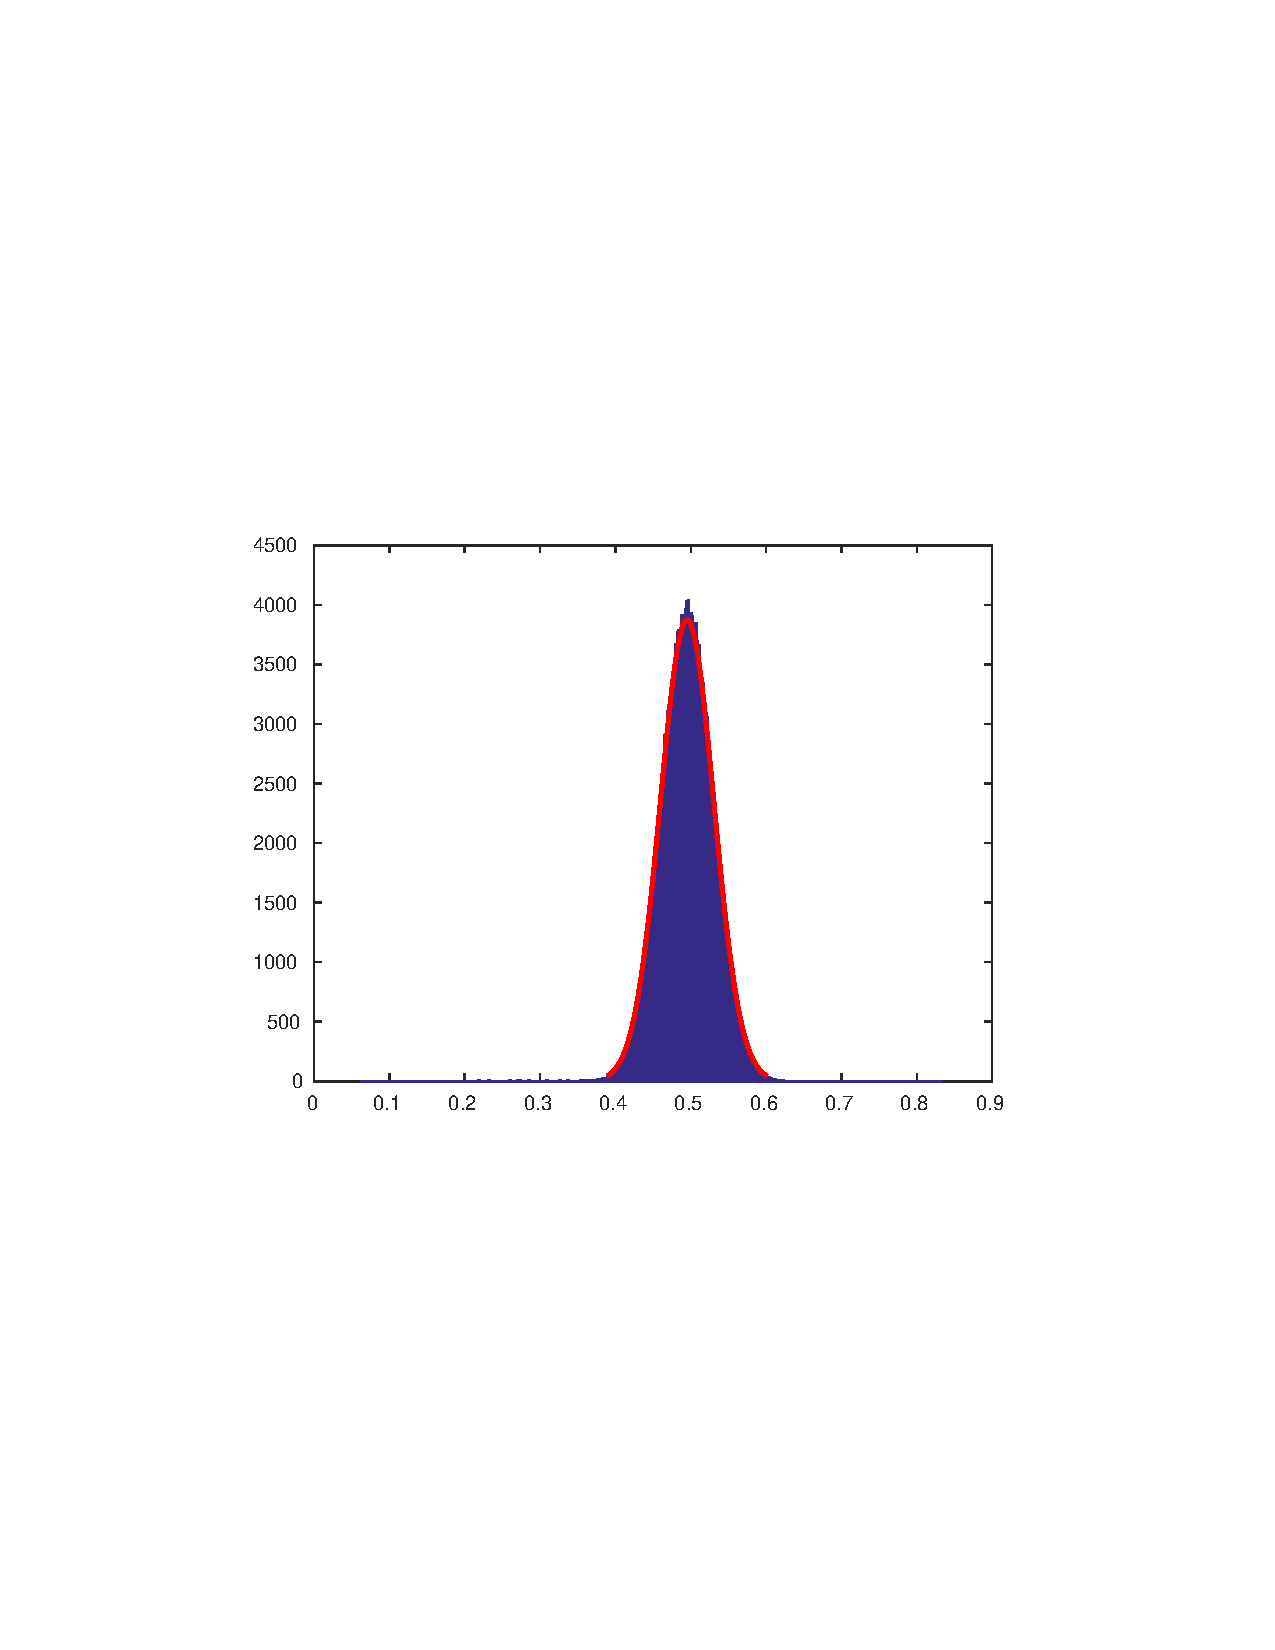
\includegraphics[width=0.9\textwidth]{imgs/theta2.pdf}
	\caption{\footnotesize Histograma de la variable $\theta_2$. La linea azul es una aproximacion con una distribución normal.}
\end{minipage}
\end{figure}

\subsection{Correlaciones}


\begin{figure}[H]
\begin{minipage}{0.5\textwidth}
 \centering
	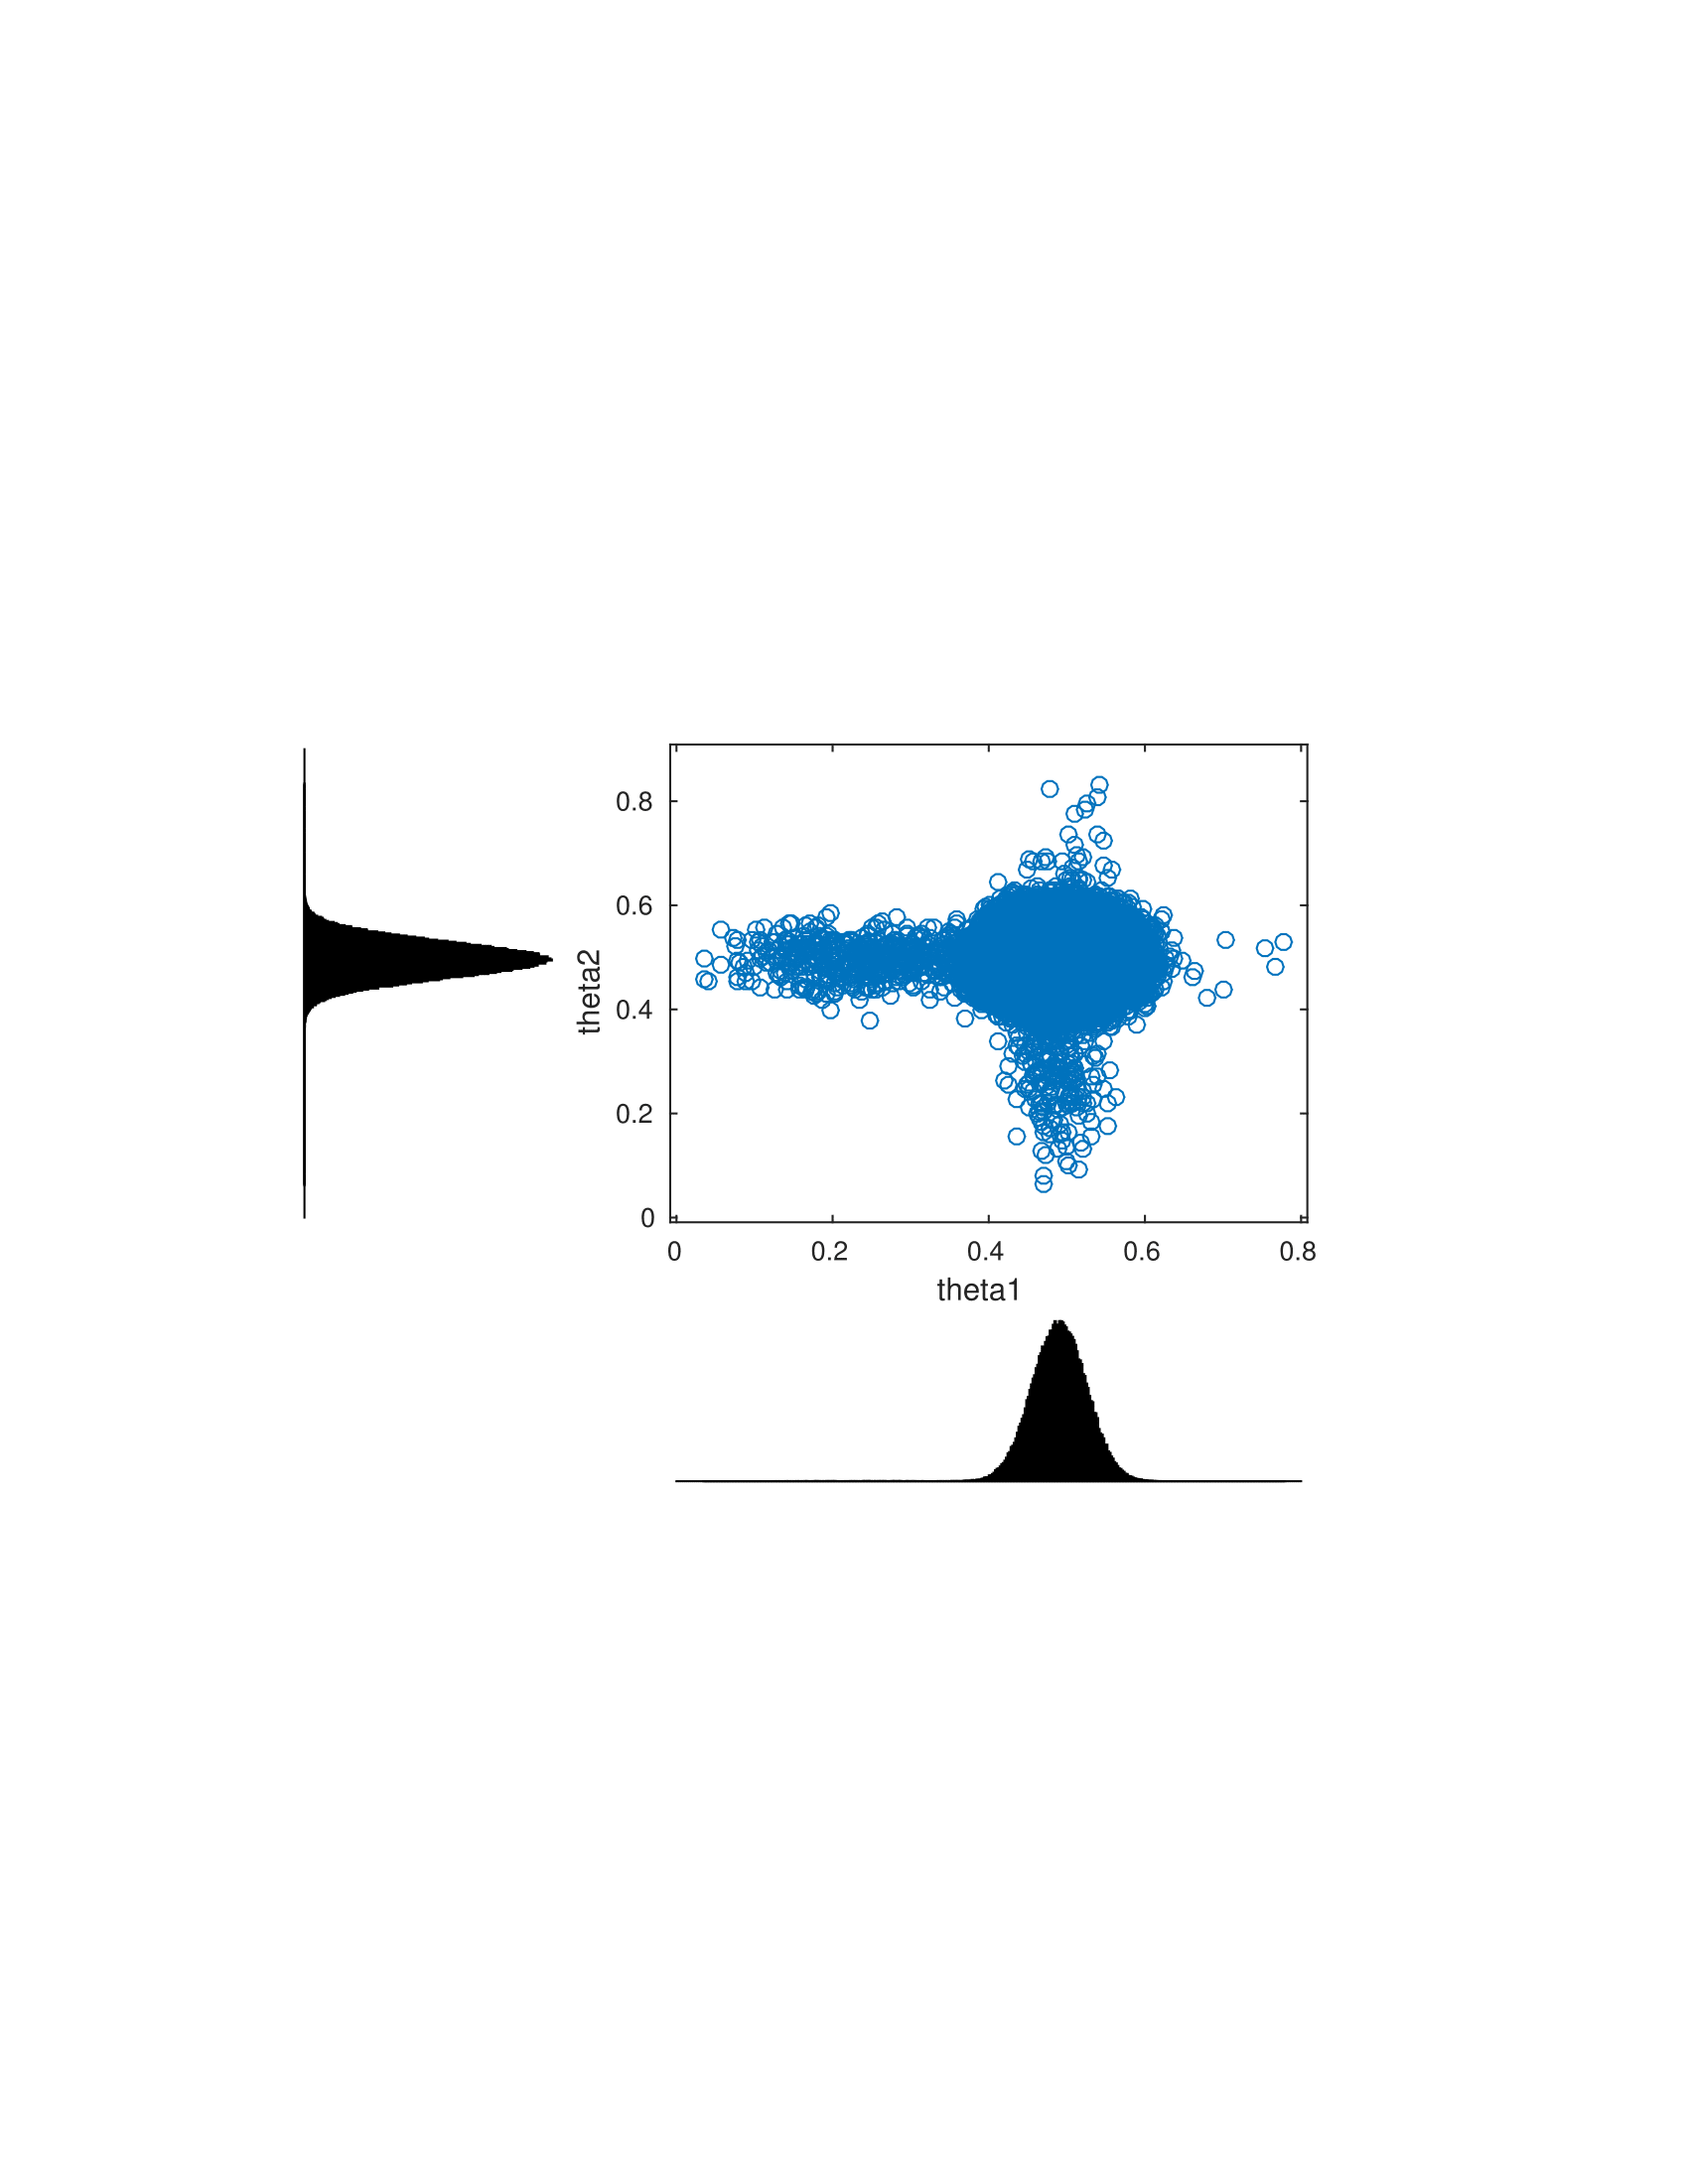
\includegraphics[width=0.9\textwidth]{imgs/theta1_2.png}
	\caption{\footnotesize Correlación entre $\theta_1$ y $\theta_2$.}
	\label{fig:problema2-promedio}
\end{minipage}
\begin{minipage}{0.5\textwidth}
 \centering
	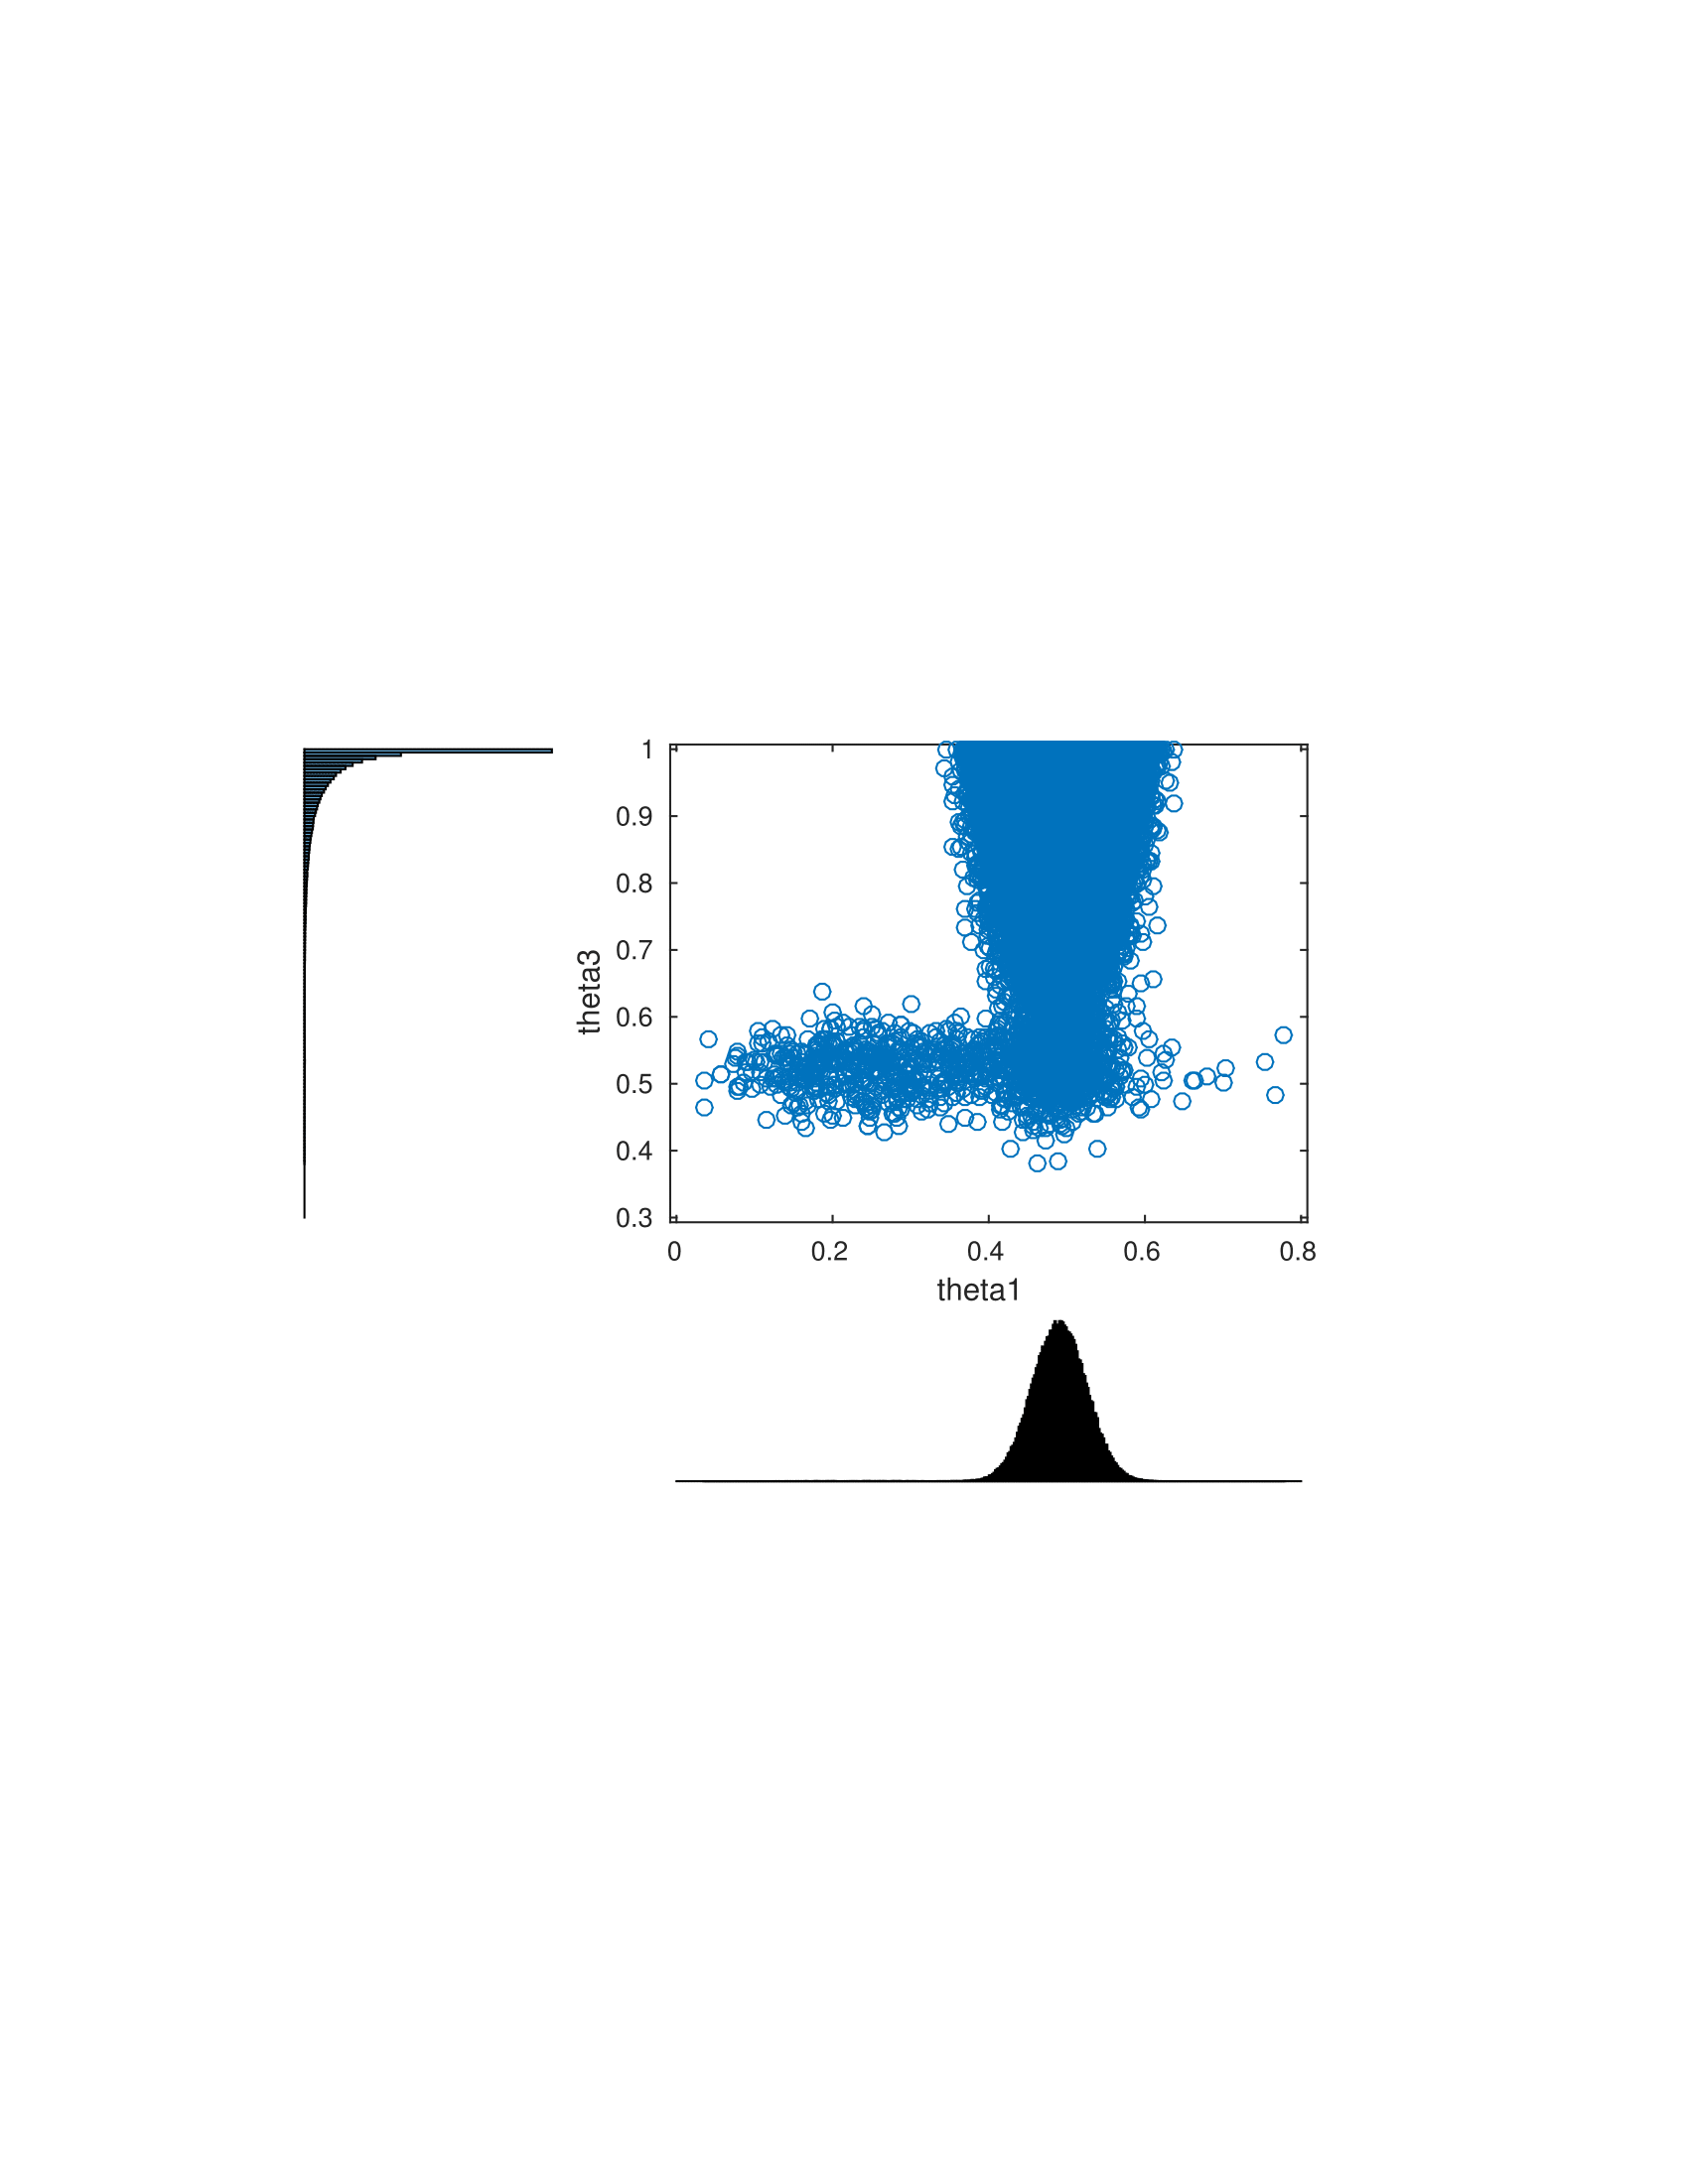
\includegraphics[width=0.9\textwidth]{imgs/theta1_3.png}
	\caption{\footnotesize Correlación entre $\theta_1$ y $\theta_2$.}
\end{minipage}
\end{figure}

\begin{figure}[H]
\centering
\begin{minipage}{0.5\textwidth}
	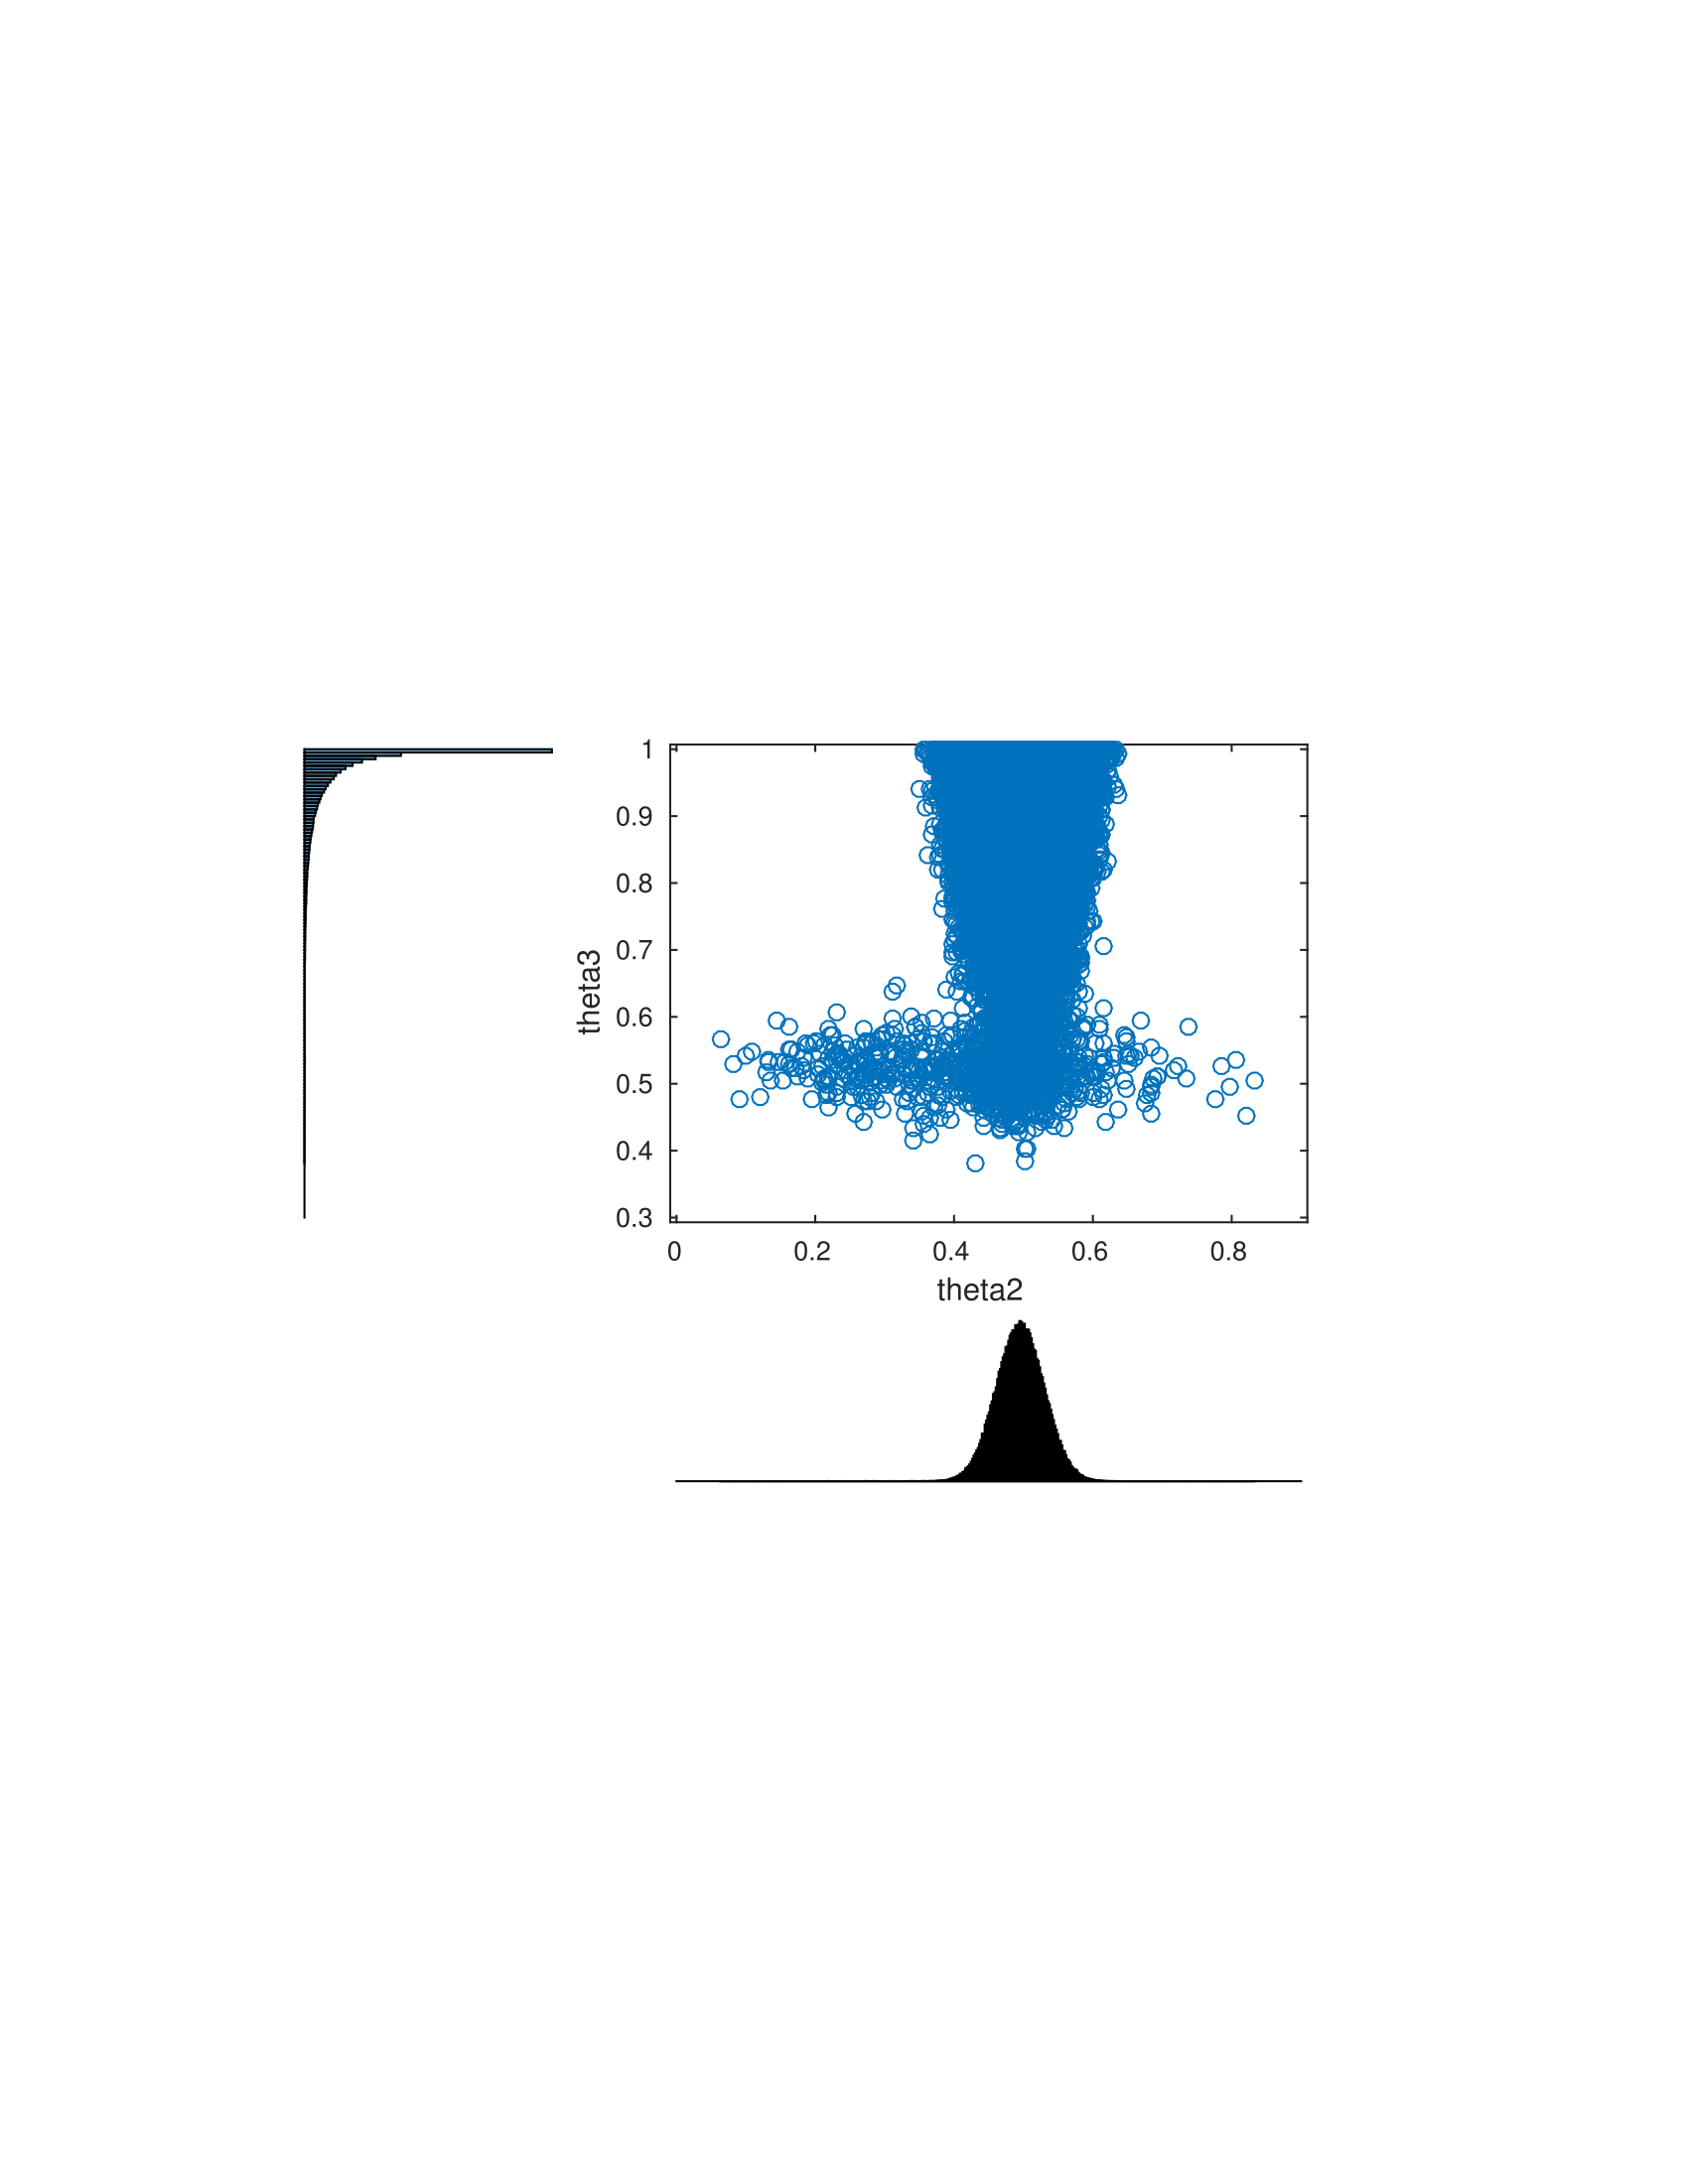
\includegraphics[width=0.9\textwidth]{imgs/theta2_3.png}
	\caption{\footnotesize Correlación entre $\theta_1$ y $\theta_2$.}
\end{minipage}	
\end{figure}


\subsection{Media y Desvío Standard}

media\_alpha = 2.9907

desvioStandard\_alpha = 0.1270

media\_t1 = 0.4899

desvioStandard\_t1 = 0.0368

media\_t2 = 0.4951

desvioStandard\_t2 = 0.0354

media\_t3 = 0.9523

desvioStandard\_t3 = 0.0680
\newpage

\section{Ejercicio 3}
\begin{figure}[H]
\begin{minipage}{0.55\textwidth}
\begin{lstlisting}[frame=single]
model{  
  # Observed Counts
  k1 ~ dbin(theta1,n)
  k2 ~ dbin(theta2,n)
  k3 ~ dbin(theta3,n)

  # Prior on Rates Theta
  theta1 ~ dbeta(param1, param1)
  theta2 ~ dbeta(param2, param2)
  theta3 ~ dbeta(param3, param3)

  # Auxiliary variables
    for Theta's distribution
  param1 <- ifelse(alpha1=1, 0.5, 100)
  param2 <- ifelse(alpha2=2, 0.5, 100)
  param3 <- ifelse(alpha3=3, 0.5, 100)

  # Prior on Rates Alpha
  alpha1 ~ dbern(0.5)  
  alpha2 ~ dbern(0.5)  
  alpha3 ~ dbern(0.5)  
}
\end{lstlisting}
\end{minipage}%
\begin{minipage}{0.45\textwidth}
\centering
\begin{tikzpicture}[>=stealth', shorten >=1pt,auto,node distance=1.9cm,
                    semithick]
  \tikzstyle{every state}=[fill=white,draw=black,text=black]

	\node[state, rectangle]	(0)							{$\alpha_2$};
	\node[state, rectangle]	(10)	[right of=0]				{$\alpha_3$};
	\node[state, rectangle]	(11)	[left of=0]				{$\alpha_1$};
	\node[state]				(1) [right of=0, below of=0]	{$\theta_3$};
	\node[state]				(3) [left of=0, below of=0]	{$\theta_1$};
	\node[state]				(2) [below of=0] 			{$\theta_2$};
	\node[state, rectangle]	(5) [below of=2, fill=gray]	{$k_2$};
	\node[state, rectangle]	(4) [below of=1, fill=gray]	{$k_3$};
	\node[state, rectangle]	(6) [below of=3, fill=gray] 	{$k_1$};
	\node[state, rectangle]	(7) [below of=5, fill=gray] 	{$n$};

	\path[->]	
    (0)  edge []	node {} (2)
    (10) edge []	node {} (1)
    (11) edge []	node {} (3)			
    (1)  edge []  node {} (4)
    (2)  edge []	node {} (5)
    (3)	 edge [] 	node {} (6)
    (7)  edge []  node {} (4)
         edge []  node {} (5)
         edge []  node {} (6);



\end{tikzpicture}
\end{minipage}%
\caption{El modelo propuesto junto con su representación gráfica.}
\label{fig:3}
\end{figure}

\newpage
\section{Ejercicio 4}
A continuación desarrollamos la expresión para la probabilidad de obtener cara en la siguiente tirada de cualquiera de las tres monedas, aprovechando la información previa. Usamos fundamentalmente las tres propiedades vistas en clase: marginalización, reescritura de la probabilidad conjunta con probabilidad condicional, y la falacia del jugador.
  \begin{equation}
  \label{eq:4}
  \begin{aligned}
	P(cara_i|D) &= \int P(cara_i, \theta_i|D) d\theta_i \\
					&= \int P(cara_i|D, \theta_i)  P(\theta_i|D) d\theta_i \\
					&= \int P(cara_i|\theta_i)  P(\theta_i|D) d\theta_i \\ 
					&= \int \theta_i  (P(\theta_i, \alpha = i|D) + P(\theta_i, \alpha \neq i|D)) d\theta_i \\
					&= \int \theta_i  (P(\theta_i | \alpha = i,D) P(\alpha = i | D) + P(\theta_i | \alpha \neq i,D) P(\alpha \neq i | D)) d\theta_i \\
  \end{aligned}
  \end{equation}

En la última línea de esta ecuación podemos identificar las siguientes fuentes de incertidumbre:
\begin{itemize}
\item La incerteza inherente al \emph{rate} de la moneda;
\item Las incerteza de la \emph{posterior} de $\theta_i$ separando en los casos en que el modelo determina que $i$ es la moneda cargada y  los que no (recordar que el \emph{prior} utilizado para $\theta_i$ es condicional a este hecho);
\item La incerteza de determinar si una moneda está cargada o no (usando la \emph{posterior} de $\alpha$).
\end{itemize}



\end{document}
